\documentclass{article}
\usepackage[T1]{fontenc}
\usepackage[utf8]{inputenc}
\usepackage{amsmath}
\usepackage{amssymb}
\usepackage{amsthm}
\usepackage{tikz}
\usetikzlibrary{arrows.meta, positioning, shapes.geometric}
\usepackage{float}
\usepackage{booktabs}

\newtheorem{definition}{Definition}
\newtheorem{remark}{Remark}

\title{Relational Emergence Model: A Generative Extension of Relational Quantum Mechanics}
\author{Yoshifumi Maruko \\ Independent Researcher, Yamagata, Japan}
\date{}

\begin{document}

\maketitle

\begin{abstract}
This paper proposes the Relational Emergence Model (REM) as a generative extension of Relational Quantum Mechanics (RQM). While RQM defines physical states as relative correlations between systems, it does not explicitly address how such correlations are dynamically produced.

The REM introduces \emph{differentiation} as a generative process through which relational distinctions become articulated and subsequently stabilized into effective classical structures via decoherence. More precisely, differentiation is formalized as a bipartition-selecting map $\mathcal{D}$---not a unitary operator, but a descriptive structural selection---that produces explicit system--observer correlations from a pre-relational Hilbert space. Environmental decoherence then suppresses off-diagonal coherences, stabilizing effectively classical facts.

Rather than asserting any equivalence between quantum theory and Buddhist philosophy, this work identifies a structural correspondence between relational quantum interpretations and the concepts of dependent origination and emptiness.

The central contribution of REM is a shift from the \emph{definition} of relational states to the \emph{modeling of the generation} of relational structure itself.
\end{abstract}

\section{Introduction}
Relational Quantum Mechanics (RQM) proposes that physical states exist only relative to other systems. While this approach removes observer-independent states, it leaves open a crucial question: how do relational structures themselves arise?

This paper introduces the Relational Emergence Model (REM), which extends RQM by providing a generative account of relational structure. Rather than treating relations as given, REM models how relational distinctions are produced through a process of differentiation.

\section{Limitations of Existing Relational Interpretations}
RQM defines states relationally but does not describe their emergence.

QBism emphasizes subjective probabilities but lacks a structural account of relational formation. Many-Worlds assumes branching structures without modeling their generative origin.

Thus, existing interpretations describe relationality but do not model its production.

\section{Relation to Recent Developments in RQM}
Recent developments in RQM have introduced important refinements, including perspectival facts, cross-perspective links, and iterative relational structures.

Adlam and Rovelli propose cross-perspective consistency, while Riedel develops the notion of iterative relationality. Weststeijn analyzes perspectival facts in Wigner-type scenarios.

However, these approaches operate on already-articulated relational structures. By contrast, REM addresses a prior question: how such relational structures become articulated in the first place.

\section{Relational Emergence Model (REM)}
\subsection{Three-Layer Architecture}
REM proposes a three-layer architecture of relational reality.

\begin{figure}[H]
\centering
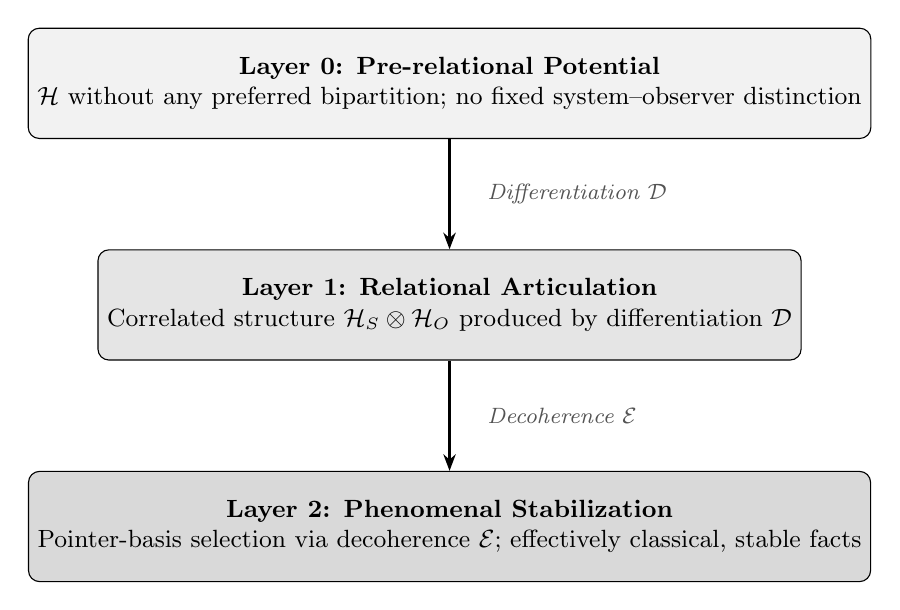
\begin{tikzpicture}[
  node distance=1.4cm,
  box/.style={rectangle, draw, rounded corners=4pt, minimum width=8.4cm, minimum height=1.4cm, align=center, font=\small},
  layer0/.style={box, fill=gray!10},
  layer1/.style={box, fill=gray!20},
  layer2/.style={box, fill=gray!30},
  arrow/.style={-{Stealth[length=6pt]}, thick},
  lbl/.style={font=\footnotesize\itshape, text=gray!65!black}
]
\node[layer0] (L0) {\textbf{Layer 0: Pre-relational Potential}\\ $\mathcal{H}$ without any preferred bipartition; no fixed system--observer distinction};
\node[layer1, below=of L0] (L1) {\textbf{Layer 1: Relational Articulation}\\ Correlated structure $\mathcal{H}_S \otimes \mathcal{H}_O$ produced by differentiation $\mathcal{D}$};
\node[layer2, below=of L1] (L2) {\textbf{Layer 2: Phenomenal Stabilization}\\ Pointer-basis selection via decoherence $\mathcal{E}$; effectively classical, stable facts};
\draw[arrow] (L0) -- (L1) node[midway, right=0.35cm, lbl] {Differentiation $\mathcal{D}$};
\draw[arrow] (L1) -- (L2) node[midway, right=0.35cm, lbl] {Decoherence $\mathcal{E}$};
\end{tikzpicture}
\caption{Three-layer architecture of REM.}
\end{figure}

\subsection{Differentiation as Generative Process}
Differentiation is defined informally as a process through which initially indistinct relational potential becomes explicitly articulated into distinguishable system--system correlations.

Observation is therefore not merely detection but the generative articulation of relational structure.

\subsection{Formal Definition of Differentiation}
\begin{definition}[Pre-relational State --- Layer~0]
Let $\mathcal{H}$ be the total Hilbert space of a composite quantum system, without any preferred tensor-product decomposition. Layer~0 corresponds to the absence of a fixed bipartition $\mathcal{H} = \mathcal{H}_S \otimes \mathcal{H}_O$.
\end{definition}

\begin{definition}[Differentiation Map --- Layer~0 $\to$ Layer~1]
A differentiation event $\mathcal{D}$ is a structural map that selects a bipartition and produces an explicit correlated state:
\[
  \mathcal{D}\colon \mathcal{H} \longrightarrow \mathcal{H}_S \otimes \mathcal{H}_O.
\]
Given a pre-relational state $\lvert\Psi\rangle \in \mathcal{H}$, differentiation yields the Schmidt decomposition
\[
  \mathcal{D}(\lvert\Psi\rangle)=\sum_i c_i\lvert s_i\rangle_S\otimes\lvert o_i\rangle_O,
  \qquad \sum_i\lvert c_i\rvert^2=1.
\]
The relational state of $S$ relative to $O$ is
\[
  \rho_{S\mid O}=\mathrm{Tr}_O\!\left(\mathcal{D}(\lvert\Psi\rangle)\mathcal{D}(\lvert\Psi\rangle)^\dagger\right).
\]
\end{definition}

\begin{remark}
$\mathcal{D}$ is not a unitary operator acting on $\mathcal{H}$. It is a descriptive bipartition-selection map: it designates which tensor-product structure is operative in a given relational context.
\end{remark}

\begin{definition}[Decoherence and Phenomenal Stabilization]
Let $\mathcal{H}_E$ denote the Hilbert space of the environment. Environmental decoherence acts as a completely positive, trace-preserving map $\mathcal{E}$ on $\rho_{S\mid O}$, suppressing off-diagonal coherences and generating effectively classical, stable, and shareable facts.
\end{definition}

\subsection{Relation to Decoherence}
Differentiation generates relational structure; decoherence stabilizes it. The ordering is strict: the decoherence map presupposes the bipartition established by $\mathcal{D}$.

\subsection{Comparison with RQM}
\begin{table}[H]
\centering
\begin{tabular}{lll}
\toprule
 & \textbf{RQM} & \textbf{REM} \\
\midrule
State Definition & Relative correlation & Relative + generative process \\
Observation & Detection / correlation & Differentiation / articulation \\
Emergence & Assumed & Modeled \\
Ontological Stance & Static relationality & Process-based relationality \\
Classicality & Decoherence & $\mathcal{D}\to\mathcal{E}$ \\
\bottomrule
\end{tabular}
\caption{Conceptual comparison of RQM and REM.}
\end{table}

\subsection{Wigner's Friend}
In REM, Wigner's Friend scenarios are interpreted as multi-level differentiation processes. Different observers correspond to different stages of relational articulation rather than contradictory descriptions of a single fixed reality.

\section{Structural Correspondence with Buddhist Philosophy}
This paper identifies a structural correspondence, not an equivalence.

Dependent origination corresponds to Layer~1, where relational structures emerge through differentiation. Emptiness corresponds to Layer~0, understood as the absence of intrinsic nature and the absence of a preferred bipartition prior to $\mathcal{D}$.

\section{Discussion}
REM introduces a generative perspective that complements existing relational interpretations of quantum mechanics.

Formalizing $\mathcal{D}$ as a bipartition-selecting map makes precise what was previously expressed only informally: observation produces rather than detects relational structure.

\section{Conclusion}
The Relational Emergence Model extends relational quantum theory by shifting the focus from the definition of relational states to the generation of relational structure itself.

By introducing differentiation as a generative, bipartition-selecting map $\mathcal{D}$ and integrating it with decoherence $\mathcal{E}$, REM provides a framework for understanding how relational reality becomes articulated and stabilized.

\begin{thebibliography}{99}
\bibitem{Rovelli1996} C.~Rovelli, ``Relational Quantum Mechanics,'' \textit{International Journal of Theoretical Physics}, 35, 1637--1678, 1996.
\bibitem{Adlam2023} E.~Adlam and C.~Rovelli, ``Information and Relational Quantum Mechanics,'' \textit{Foundations of Physics}, 53, 2023.
\bibitem{Riedel2024} C.~J.~Riedel, ``Iterated Relational Quantum Mechanics,'' 2024.
\bibitem{Weststeijn2021} W.~Weststeijn, ``Perspectival Facts in Quantum Mechanics,'' 2021.
\bibitem{FrauchigerRenner2018} D.~Frauchiger and R.~Renner, ``Quantum theory cannot consistently describe the use of itself,'' \textit{Nature Communications}, 9, 3711, 2018.
\bibitem{Brukner2018} \v{C}.~Brukner, ``A no-go theorem for observer-independent facts,'' \textit{Entropy}, 20, 350, 2018.
\bibitem{SpencerBrown1969} G.~Spencer-Brown, \textit{Laws of Form}. George Allen and Unwin, 1969.
\bibitem{Garfield1995} J.~L.~Garfield, \textit{The Fundamental Wisdom of the Middle Way}. Oxford University Press, 1995.
\bibitem{Siderits2007} M.~Siderits, \textit{Buddhism as Philosophy}. Hackett Publishing, 2007.
\bibitem{CalosiRiedel2024} C.~Calosi and C.~Riedel, ``Relational Structure in Quantum Mechanics,'' 2024.
\end{thebibliography}

\end{document}
